\subsection{Анализ с испольнованием нейросетей}
\label{sec:analogues:neural}

Приведенный выше анализ существующих типов нейронных сетей позволяет сделать вывод, что целесообразным является
использование нейронной сети для задачи прогнозирования, обучение с учителем с применением алгоритма обратного
распространения ошибки.

Данное удтверждение подтверждается анализом статьи~\cite{using_neural_engines}. В данной статье проведено
исследование и разработка методики оценки стоимости \linebreak недвижимости с использованием нейросетевых технологий. Были решены
задачи предварительного отбора факторов, оказывающих влияние на рыночную стоимость квартир; подготовлена обучающая выборка
и определены оптимальные типы и характеристики, а также метода ее обученииия.

Обучающая выборка построена для проектирования и обучения нейронной сети «с учителем», к реализации
предполагается 3 типа сетей: многослойный персептрон (MLP); сеть радиально-базисных функций (RBF);\linebreak
обобщенно-регрессионная нейронная сеть (GRNN).

Многослойный персептрон - это класс искусственных нейронных сетей прямого распространения, состоящих как минимум из
трех слоёв: входного, скрытого и выходного. За исключением входных, все нейроны использует нелинейную функцию активации.

При обучении MLP используется обучение с учителем и алгоритм обратного распространения ошибки.

Обобщенная схема многослойного перспетрона показана на \linebreak рисунке~\ref{fig:analogues:multilayer-neural-net}

\begin{figure}[!ht]
  \centering
  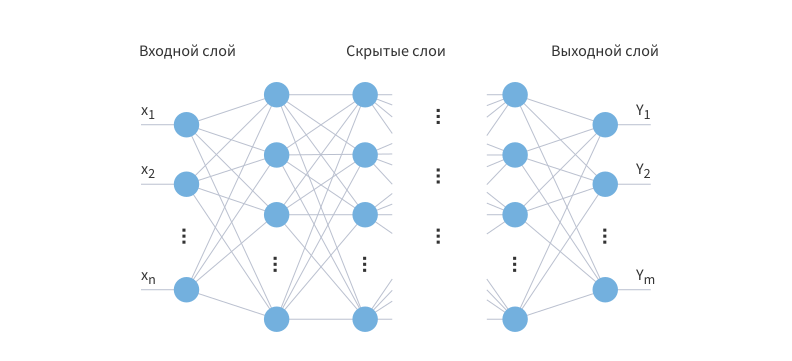
\includegraphics[scale=0.65]{multilayer-neural-net.png} 
  \caption{Схема многослойного перспетрона}
  \label{fig:analogues:multilayer-neural-net}
\end{figure}

В качестве активационных функций нейронов используются сигмоидальные: логистическая или гиперболический тангенс.

MLP показали возможность находить приближённые решения для чрезвычайно сложных задач. В частности, они являются
универсальным аппроксиматором функций, поэтому с успехом используются в построении регрессионных моделей.
Поскольку классификацию можно рассматривать как частный случай регрессии, когда выходная переменная категориальная,
на основе MLP можно строить классификаторы.

Пик популярности MLP в машинном обучении пришёлся на 1980-е годы в таких областях, как распознавание речи и
изображений, системах машинного перевода. Однако позднее они столкнулись с конкуренцией с другими технологиями
машинного обучения, такими, как машины опорных векторов. Интерес к многослойным персептронам вернулся благодаря
успехам глубокого обучения.

Радиально-симметричные функции – простейший класс функций. \linebreak В принципе, они могут быть использованы в разных моделях
(линейных и нелинейных) и в разных сетях (многослойных и однослойных). Традиционно термин RBF сети ассоциируется с
радиально-симметричными функциями в однослойных сетях, имеющих структуру, представленную на рисунке~\ref{fig:analogues:rbf-network}.

\begin{figure}[!ht]
  \centering
  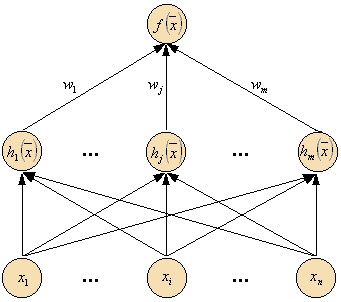
\includegraphics[scale=1]{rbf-network.png} 
  \caption{Схема RBF сети}
  \label{fig:analogues:rbf-network}
\end{figure}

То есть, каждый из n компонентов входного вектора подается на вход m базисных функций и их выходы линейно суммируются
с весами.

Обобщенно-регрессионная нейронная сеть (GRNN) устроена аналогично вероятностной нейронной сети (PNN), но она
предназначена для решения задач регрессии, а не классификации. Обобщенная схема GRNN сети представлена на
рисунке~\ref{fig:analogues:grnn-network}. Как и в случае PNN-сети, в точку расположения каждого
обучающего наблюдения помещается гауссова ядерная функция. Мы считаем, что каждое наблюдение свидетельствует о
некоторой нашей уверенности в том, что поверхность отклика в данной точке имеет определенную высоту, и эта
уверенность убывает при отходе в сторону от точки. GRNN-сеть копирует внутрь себя все обучающие наблюдения и
использует их для оценки отклика в произвольной точке. Окончательная выходная оценка сети получается как взвешенное
среднее выходов по всем обучающим наблюдениям, где величины весов отражают расстояние от этих наблюдений до той точки,
в которой производится оценивание (и, таким образом, более близкие точки вносят больший вклад в оценку).

\begin{figure}[!ht]
  \centering
  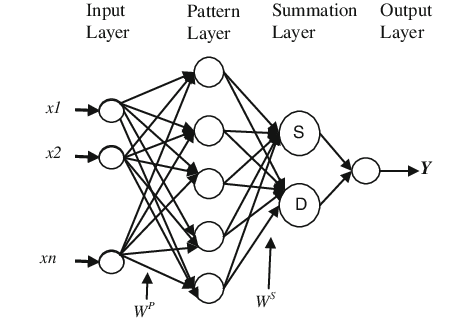
\includegraphics[scale=1.6]{grnn-network.png} 
  \caption{Схема GRNN сети}
  \label{fig:analogues:grnn-network}
\end{figure}

Первый промежуточный слой сети GRNN состоит из радиальных элементов. Второй промежуточный слой содержит элементы,
которые помогают оценить взвешенное среднее. Для этого используется специальная процедура. Каждый выход имеет в этом
слое свой элемент, формирующий для него взвешенную сумму. Чтобы получить из взвешенной суммы взвешенное среднее, эту
сумму нужно поделить на сумму весовых коэффициентов. Последнюю сумму вычисляет специальный элемент второго слоя.
После этого в выходном слое производится собственно деление (с помощью специальных элементов "деления"). Таким
образом, число элементов во втором промежуточном слое на единицу больше, чем в выходном слое. Как правило, в задачах
регрессии требуется оценить одно выходное значение, и, соответственно, второй промежуточный слой содержит два элемента.

Можно модифицировать GRNN-сеть таким образом, чтобы радиальные элементы соответствовали не отдельным обучающим
случаям, а их кластерам. Это уменьшает размеры сети и увеличивает скорость обучения. Центры для таких элементов
можно выбирать с помощью любого предназначенного для этой цели алгоритма (выборки из выборки, K-средних или Кохонена).

GRNN-сеть обучается почти мгновенно, но может получиться большой и медленной (хотя здесь, в отличие от PNN, не
обязательно иметь по одному радиальному элементу на каждый обучающий пример, их число все равно будет большим).
Как и сеть RBF, сеть GRNN не обладает способностью экстраполировать данные.

Проведенное сравнение полученных результатов(рис.~\ref{fig:analogues:comparing}),
полученных в статье~\cite{using_neural_engines} позволяет сделать выводы.

\begin{figure}[!ht]
  \centering
  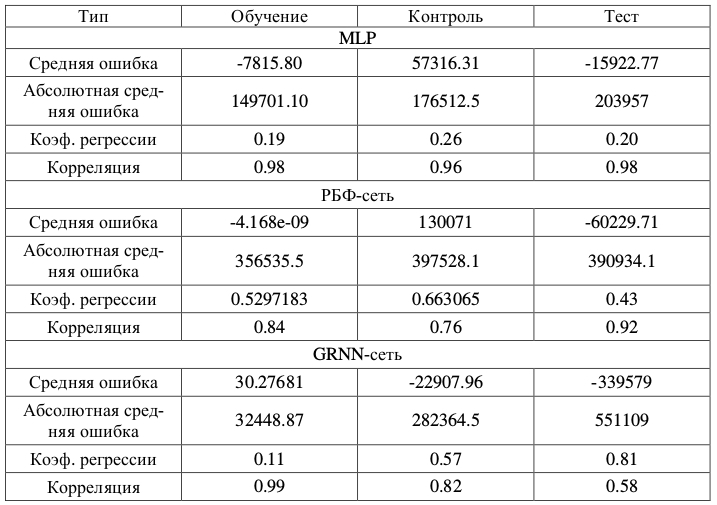
\includegraphics[scale=0.65]{comparing.jpg} 
  \caption{Сравнение полученных результатов}
  \label{fig:analogues:comparing}
\end{figure}

GRNN-сеть показала очень хорошие результаты на тестовой выборке, в то время как на тестовой выборке ее эффективность
оказалась значительно ниже, чем у прочих рассмотренных сетей. Наиболее вероятным здесь событием является нерешенная
проблема переобучения. То есть минимизировалась не та ошибка, которая ожидается от сети при подаче совершенно новых
значений. Другими словами, у данной сети отсутствует способность обобщать результаты работы на новые наблюдения.

РБФ-сеть не продемонстрировала высоких результатов, однако несомненным ее достоинством является более высокая скорость
обучения.

Многослойный персептрон является наиболее подходящим вариантом решения задачи определения стоимости жилых квартир.
Полученные данные позволяют с достаточной точностью прогнозировать стоимость квартир по заданным параметрам.

Среди достоинств данной статьи, которые будут использованы при проведении эксперимента,
можно отметить построение нескольких типов нейронных сетей и дальнейшее сравнение их результатов.
Рассмотрены и реализованы 3 типа сетей: многослойный персептрон (MLP); сеть радиально-базисных функций (RBF);
обобщенно-регрессионная нейронная сеть (GRNN). Многослойный персептрон является наиболее подходящим вариантом решения
задачи определения стоимости жилых квартир.

Среди недостатков данной статьи, которые предполагается устранить, можно отметить небольшой объем выборки, а также 
построение нескольких моделей отдельно по какому-либо признаку. Увеличение объема выборки и построение отдельных сетей
должно повысить качетсво получаемых результатов.
